\documentclass[10pt, a4paper]{article}

\usepackage{amsmath}
\usepackage{amssymb}
\usepackage{graphicx}
\usepackage{listings}
\usepackage{color}
\usepackage[section]{placeins}
\usepackage{paralist}

\definecolor{mygreen}{rgb}{0,0.6,0}
\definecolor{mygray}{rgb}{0.5,0.5,0.5}
\definecolor{mymauve}{rgb}{0.58,0,0.82}

\lstset{ %
  backgroundcolor=\color{white},
  basicstyle=\footnotesize,
  breakatwhitespace=false,
  breaklines=true,
  captionpos=b,
  commentstyle=\color{mygreen},
  escapeinside={\%*}{*)},
  extendedchars=true,
  keepspaces=true,
  keywordstyle=\color{blue},
  rulecolor=\color{black},
  showspaces=false,
  showstringspaces=false,
  showtabs=false,
  stepnumber=2,
  stringstyle=\color{mymauve},
  tabsize=2,
}

\hyphenation{GENITOR}

\newcommand*{\titleGM}{\begingroup
\hbox{ 
\hspace*{0.2\textwidth} 
\rule{1pt}{\textheight} 
\hspace*{0.05\textwidth} 
\parbox[b]{0.75\textwidth}{ 

{\noindent\Huge\bfseries Solving Travelling Salesman Problems using Genetic
 Algorithms}\\[2\baselineskip] % Title
{\large \textit{SEM6120 - Assignment 2}}\\[4\baselineskip] % Tagline or further description
{\Large \textsc{Alexander D Brown (adb9)}} % Author name

\vspace{0.5\textheight} 
}}
\endgroup}


\title{Genetic Algorithms}
\author{Alexander D Brown (adb9)}

\begin{document}
\titleGM 
\tableofcontents
\newpage

\section{Design}

\subsection{UML Class Diagram}

Figure~\ref{fig:uml} shows the initial UML Class diagram for this project.
There are some elements which break from typical object-orientated design,
noticeably the representation of nodes in a graph as a map of integers to a
turple of float, these parts are done so to re-use internal data structures of
the Python programming language to speed up the implementation of many 
features.

\begin{figure}[h]
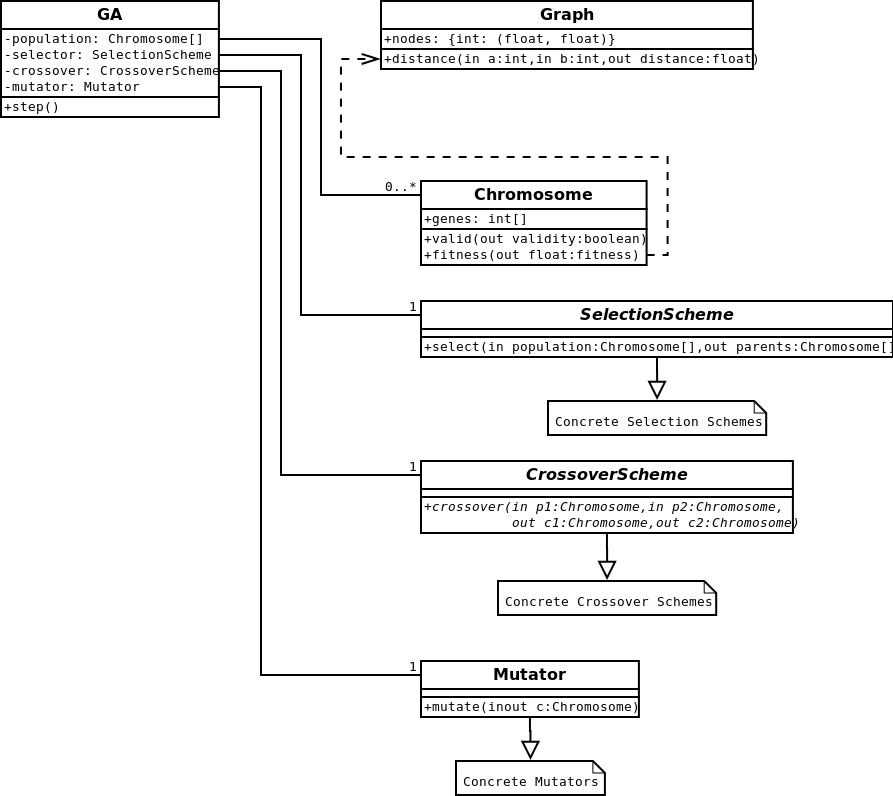
\includegraphics[width=\textwidth]{img/uml.png}
\caption{UML Class Diagram for the Genetic Algorithm}
\label{fig:uml}
\end{figure}

This design is such that factories exist to create selection schemes, crossover
schemes and mutators based on an input string to facilitate the switching of
these elements via command line arguments.

This design was slowly improved through the project; the
\texttt{CrossoverScheme} class implemented the \texttt{crossover} method, 
which then called a separate method, \texttt{do\_crossover}, to generate 
\texttt{c1} based on \texttt{do\_crossover(p1, p2)} and \texttt{c2} on 
\texttt{do\_crossover(p2, p1)} to make the processing more uniform. Subclasses
were still able to override the \texttt{crossover} method, but were encouraged
to implement a \texttt{do\_crossover} method unless the scheme required a
different behaviour of child generation.


\subsection{Representation of Graphs}

The actual of representation of a graph is a map of the node identifier to the
$x$ and $y$ co-ordinates of that node (as a turple). This allows easy look up 
of nodes within the map to get the position of the node. This was chosen 
because of the representation of the problem in chromosomes - each gene 
represents a node in the graph.

With this representation, the fitness function would be the distance of the 
tour represented by these nodes:

\begin{equation}
d_{tour} = \sum^{N}_{i=0}{
  \begin{cases}
    d(n_i, n_{i+1}) & \text{if } i+n < N \\ 
    d(n_i, n_0)     & \text{else}
  \end{cases}
}
\end{equation}

Programatically, with the advantage of the functional and in-built elements of 
Python, this can be simplified to:

\lstset{language=Python}
\begin{lstlisting}[language=Python, caption=Distance of a tour]
def d_tour():
  # Move the first element of the array to the end.
  shifted = nodes[1:] + nodes[:1]
  return sum([distance(i, j) for (i, j) in zip(nodes, shifted)])
\end{lstlisting}

\subsection{Use of Functional Programming Paradigms}

As Python implements several different programming paradigms a lot of problems
can be solved with a different approach than other languages can. Both genetic
algorithms and the travelling salesman problem lend themselves towards a more
functional approach with a lot of list processing. Using Pythons list
comprehensions and the in-built list functions shortened the amount of code 
required and makes the code a lot easier to understand for those who are used 
to this approach.

A very good example of this is the method for evaluating chromosomes in a
population, returning a list sorted from the best to the worst:

\begin{lstlisting}[language=Python, 
                   caption=Using function elements to improve sustinctness and
                           readability]
def eval(population):
  return sorted(map(eval_single, population), 
                key = lambda chromosome: chromosome.score)

def eval_single(chromosome):
  chromosome.score = chromosome.fitness()
  return chromosome
\end{lstlisting}


\end{document}
